% Options for packages loaded elsewhere
\PassOptionsToPackage{unicode}{hyperref}
\PassOptionsToPackage{hyphens}{url}
\documentclass[
  ignorenonframetext,
]{beamer}
\newif\ifbibliography
\usepackage{pgfpages}
\setbeamertemplate{caption}[numbered]
\setbeamertemplate{caption label separator}{: }
\setbeamercolor{caption name}{fg=normal text.fg}
\beamertemplatenavigationsymbolsempty
% remove section numbering
\setbeamertemplate{part page}{
  \centering
  \begin{beamercolorbox}[sep=16pt,center]{part title}
    \usebeamerfont{part title}\insertpart\par
  \end{beamercolorbox}
}
\setbeamertemplate{section page}{
  \centering
  \begin{beamercolorbox}[sep=12pt,center]{section title}
    \usebeamerfont{section title}\insertsection\par
  \end{beamercolorbox}
}
\setbeamertemplate{subsection page}{
  \centering
  \begin{beamercolorbox}[sep=8pt,center]{subsection title}
    \usebeamerfont{subsection title}\insertsubsection\par
  \end{beamercolorbox}
}
% Prevent slide breaks in the middle of a paragraph
\widowpenalties 1 10000
\raggedbottom
\AtBeginPart{
  \frame{\partpage}
}
\AtBeginSection{
  \ifbibliography
  \else
    \frame{\sectionpage}
  \fi
}
\AtBeginSubsection{
  \frame{\subsectionpage}
}
\usepackage{iftex}
\ifPDFTeX
  \usepackage[T1]{fontenc}
  \usepackage[utf8]{inputenc}
  \usepackage{textcomp} % provide euro and other symbols
\else % if luatex or xetex
  \usepackage{unicode-math} % this also loads fontspec
  \defaultfontfeatures{Scale=MatchLowercase}
  \defaultfontfeatures[\rmfamily]{Ligatures=TeX,Scale=1}
\fi
\usepackage{lmodern}
\ifPDFTeX\else
  % xetex/luatex font selection
\fi
% Use upquote if available, for straight quotes in verbatim environments
\IfFileExists{upquote.sty}{\usepackage{upquote}}{}
\IfFileExists{microtype.sty}{% use microtype if available
  \usepackage[]{microtype}
  \UseMicrotypeSet[protrusion]{basicmath} % disable protrusion for tt fonts
}{}
\makeatletter
\@ifundefined{KOMAClassName}{% if non-KOMA class
  \IfFileExists{parskip.sty}{%
    \usepackage{parskip}
  }{% else
    \setlength{\parindent}{0pt}
    \setlength{\parskip}{6pt plus 2pt minus 1pt}}
}{% if KOMA class
  \KOMAoptions{parskip=half}}
\makeatother
\usepackage{longtable,booktabs,array}
\newcounter{none} % for unnumbered tables
\usepackage{calc} % for calculating minipage widths
\usepackage{caption}
% Make caption package work with longtable
\makeatletter
\def\fnum@table{\tablename~\thetable}
\makeatother
\usepackage{graphicx}
\makeatletter
\newsavebox\pandoc@box
\newcommand*\pandocbounded[1]{% scales image to fit in text height/width
  \sbox\pandoc@box{#1}%
  \Gscale@div\@tempa{\textheight}{\dimexpr\ht\pandoc@box+\dp\pandoc@box\relax}%
  \Gscale@div\@tempb{\linewidth}{\wd\pandoc@box}%
  \ifdim\@tempb\p@<\@tempa\p@\let\@tempa\@tempb\fi% select the smaller of both
  \ifdim\@tempa\p@<\p@\scalebox{\@tempa}{\usebox\pandoc@box}%
  \else\usebox{\pandoc@box}%
  \fi%
}
% Set default figure placement to htbp
\def\fps@figure{htbp}
\makeatother
\setlength{\emergencystretch}{3em} % prevent overfull lines
\providecommand{\tightlist}{%
  \setlength{\itemsep}{0pt}\setlength{\parskip}{0pt}}
% Auto-generated by infrastructure/rendering/_pdf_latex_helpers.py::extract_math_font_preamble.
% Minimal header passed to Pandoc via -H so Beamer slides pick up the same math font
% as the combined-PDF path. Adjust the manuscript's preamble.md to change the font globally.
\usepackage{unicode-math}
\setmathfont{latinmodern-math.otf}
\usepackage{bookmark}
\IfFileExists{xurl.sty}{\usepackage{xurl}}{} % add URL line breaks if available
\urlstyle{same}
\hypersetup{
  hidelinks,
  pdfcreator={LaTeX via pandoc}}

\author{\texorpdfstring{}{}}
\date{}

\begin{document}

\section{Case Subscripts, Passivization, and the Curry--Howard
Proof}\label{sec:case-type-logic}

\begin{frame}[allowframebreaks]{Case Subscripts, Passivization, and the
Curry--Howard Proof}
\textbf{Where we are in the argument.} \autoref{sec:categorial-grammar}
installed pregroup syntax --- cups, caps, and compact closure --- as the
algebraic backbone of composition. This chapter decorates that backbone
with case information: every noun wire picks up a case subscript
(\(n_{\text{NOM}}\), \(n_{\text{ACC}}\), \ldots) so grammatical role
becomes a first-class typed structure on wires, and passivization
becomes a wire-level swap together with \textbf{case relabeling}
(\autoref{eq:eq-3-3}/\autoref{eq:eq-3-4}) rather than an exception to
the type system --- the Curry--Howard image is a proof rewrite of that
rearrangement.

Case-marked noun phrases receive compound types that encode both their
grammatical role and their combinatory potential. For example, in a
nominative--accusative language, the type assignment proceeds as follows
(\autoref{tbl:pregroup-types}):

\begin{longtable}[]{@{}
  >{\raggedright\arraybackslash}p{(\linewidth - 4\tabcolsep) * \real{0.3333}}
  >{\raggedright\arraybackslash}p{(\linewidth - 4\tabcolsep) * \real{0.3333}}
  >{\raggedright\arraybackslash}p{(\linewidth - 4\tabcolsep) * \real{0.3333}}@{}}
\caption{Case-marked pregroup type assignments for a standard
nominative-accusative transitive
clause.}\label{tbl:pregroup-types}\tabularnewline
\toprule\noalign{}
\begin{minipage}[b]{\linewidth}\raggedright
Expression
\end{minipage} & \begin{minipage}[b]{\linewidth}\raggedright
Type
\end{minipage} & \begin{minipage}[b]{\linewidth}\raggedright
Gloss
\end{minipage} \\
\midrule\noalign{}
\endfirsthead
\toprule\noalign{}
\begin{minipage}[b]{\linewidth}\raggedright
Expression
\end{minipage} & \begin{minipage}[b]{\linewidth}\raggedright
Type
\end{minipage} & \begin{minipage}[b]{\linewidth}\raggedright
Gloss
\end{minipage} \\
\midrule\noalign{}
\endhead
``Alice'' (subject) & \(n_{\text{NOM}}\) & Noun, nominative-marked \\
``the ball'' (object) & \(n_{\text{ACC}}\) & Noun, accusative-marked \\
``kicks'' & \((n_{\text{NOM}} \backslash s) / n_{\text{ACC}}\) & Seeks
ACC right, NOM left \\
``to Bob'' (recipient) & \((s \backslash s) / n_{\text{DAT}}\) &
Modifies sentence via DAT argument \\
\bottomrule\noalign{}
\end{longtable}

The specific subscripts structurally refine the base noun type \(n\)
with mandatory continuous case features, mathematically guaranteeing
that the transitive verb ``kicks'' exclusively selects a
nominative-marked subject and an accusative-marked object. Any feature
mismatch automatically blocks the algebraic derivation, accurately
modeling native ungrammaticality.

\textbf{Alignment and natural transformations.} Cross-linguistic
alignment is modeled functorially in \autoref{sec:case-categories}:
alignment types are structure-preserving functors from a universal role
category to a language-specific case category, compared via natural
transformations when one asks how two alignments cohere on the same
underlying argument structure. At the level of case-marked pregroup
types (this section), that functorial picture \textbf{suggests} treating
agreement checks as naturality-style coherence constraints: the
morphosyntactic alignment chosen for arguments must remain compatible
with the verb's combinatorial requirements so that reductions still
factor through the intended case-typed slots. We do not claim a full
adjunction between identity and alignment functors in the pregroup
category here; the precise categorical status of alignment is anchored
in \autoref{sec:case-categories}, while the typed reductions below
supply the concrete syntax.
\end{frame}

\begin{frame}[allowframebreaks]{Syntactic Derivation as Proof, Case
Assignment as Type Inference}
\protect\phantomsection\label{syntactic-derivation-as-proof-case-assignment-as-type-inference}
A deep structural parallel underlies the Lambek calculus: derivations of
syntactic types correspond to proofs in intuitionistic logic (via the
Curry--Howard isomorphism), and therefore to programs in a typed lambda
calculus, as summarized in \autoref{tbl:curry-howard}.

\begin{longtable}[]{@{}
  >{\raggedright\arraybackslash}p{(\linewidth - 4\tabcolsep) * \real{0.3333}}
  >{\raggedright\arraybackslash}p{(\linewidth - 4\tabcolsep) * \real{0.3333}}
  >{\raggedright\arraybackslash}p{(\linewidth - 4\tabcolsep) * \real{0.3333}}@{}}
\caption{The Curry--Howard isomorphism connecting syntactic, logical,
and computational domains.}\label{tbl:curry-howard}\tabularnewline
\toprule\noalign{}
\begin{minipage}[b]{\linewidth}\raggedright
Syntactic Domain
\end{minipage} & \begin{minipage}[b]{\linewidth}\raggedright
Logical Domain
\end{minipage} & \begin{minipage}[b]{\linewidth}\raggedright
Computational Domain
\end{minipage} \\
\midrule\noalign{}
\endfirsthead
\toprule\noalign{}
\begin{minipage}[b]{\linewidth}\raggedright
Syntactic Domain
\end{minipage} & \begin{minipage}[b]{\linewidth}\raggedright
Logical Domain
\end{minipage} & \begin{minipage}[b]{\linewidth}\raggedright
Computational Domain
\end{minipage} \\
\midrule\noalign{}
\endhead
Types \((A / B, A \backslash B)\) & Propositions & Types \\
Derivations & Proofs & Programs (\(\lambda\text{-terms}\)) \\
Cut elimination & Proof normalization & \(\beta\text{-reduction}\) \\
Commutativity of cuts & Confluence of rewriting & Church--Rosser
property \\
\bottomrule\noalign{}
\end{longtable}

This foundational correspondence dictates two critical consequences for
our cognitive framework:

\begin{enumerate}
\tightlist
\item
  \textbf{Semantic compositionality strictly follows syntactic
  well-formedness}: A successfully typed derivation automatically
  guarantees a well-formed geometric meaning representation
  (specifically, the exact \(\lambda\text{-term}\) isolated and
  extracted directly from the formal proof).
\item
  \textbf{Case assignment reduces to type inference}: Dynamically
  determining the correct case for a noun phrase in context is
  computationally equivalent to inferring the type of an unknown
  variable in a \(\lambda\text{-expression}\)---thereby grounding case
  assignment in the well-understood algorithmic landscape of type
  inference (Hindley-Milner and its extensions).
\end{enumerate}
\end{frame}

\begin{frame}[allowframebreaks]{Song's Monadic Root Syntax: Sublexical
Decomposition via Embedded Monads}
\protect\phantomsection\label{songs-monadic-root-syntax-sublexical-decomposition-via-embedded-monads}
Song {[}-@song2022act; -@song2022blog{]} significantly extends this
categorial framework by deploying a novel \textbf{monadic semantics} for
root syntax. He successfully models the sublexical decomposition of
complex verb roots by embedding specialized monads directly into the
base syntactic category. This computational approach captures the deep
intuition that a seemingly simple verb like ``break'' harbors layered
internal structure---specifically, an active causative layer tightly
coupled to a passive result-state layer---which dynamically dictates
subsequent case assignment. The formal monad elegantly encapsulates this
tangled lexical complexity within one streamlined categorical
construction, empowering the type-logical grammar to process lexical
features and syntactic composition simultaneously and uniformly.

This monadic architecture seamlessly interfaces with modern graded type
theory. For instance, Asudeh and Giorgolo {[}-@asudeh2020graded{]}
previously developed a monadic semantics tracking evidentiality,
deploying graded computational effects to quantify the shifting
epistemic real-world status of various propositions. Our framework
extends this exact pattern into the domain of morphological case, where
the continuous ``grade'' attached to any specific morphism formally
encodes the statistical strength and validity of that local semantic
role assignment.
\end{frame}

\begin{frame}[fragile,allowframebreaks]{Passivization Is a Swap: Voice
Alternation as Topological Wire Crossing}
\protect\phantomsection\label{passivization-is-a-swap-voice-alternation-as-topological-wire-crossing}
Within categorical linguistics, \textbf{passivization} emerges as a
uniquely revealing topological operation. Traditionally described as a
syntactic rule that promotes the patient to subject position while
(optionally) demoting the agent to an oblique role, passivization in our
framework ceases to be an ad-hoc transformation; instead, it combines
(i) a \textbf{Swap} morphism
\(\sigma_{A,B}: A \otimes B \to B \otimes A\) that crosses the noun
wires feeding into the verb's pregroup derivation---so \emph{which} noun
meets the verb's left vs.~right adjoint slots reverses relative to the
active diagram---and (ii) \textbf{updated case features} on those wires:
the promoted subject is \(n_{\text{NOM}}\), not a carried-over
\(n_{\text{ACC}}\).

In a pregroup grammar, the active transitive ``Alice chases Bob'' has
the type reduction:

\begin{equation}
n_{\text{NOM}} \cdot (n^r \cdot s \cdot n^l) \cdot n_{\text{ACC}} \to s
\label{eq:eq-3-3}
\end{equation}

For ``Bob is chased by Alice,'' Bob is the grammatical subject
(\(n_{\text{NOM}}\)) and Alice appears in the oblique \emph{by}-phrase
(\(n_{\text{OBL}}\)), with surface order subject--verb--oblique:

\begin{equation}
n_{\text{NOM}} \cdot (n^r \cdot s \cdot n^l) \cdot n_{\text{OBL}} \to s
\label{eq:eq-3-4}
\end{equation}

This is \textbf{not} the naive swap of subscripts in \eqref{eq:eq-3-3}
(which would incorrectly leave the promoted patient typed as
accusative). The DisCoPy \texttt{Swap} primitive makes the wire crossing
explicit; the case-marked types in \eqref{eq:eq-3-4} match the figure
and standard promotion/demotion. The generated passive diagram diverges
from its active counterpart through that crossing together with the
reassignment of which noun occupies each cup. This transforms abstract
syntactic voice alternation into a highly visible, instantly readable
topological feature embedded directly within the string diagram.

This diagrammatic transparency exemplifies Shimojima's
{[}-@shimojima1996reasoning{]} free-ride inference capability. By
inspecting the visual topology, a cognitive agent immediately verifies
that passivization preserves the verb's inherent argument structure
while rearranging its surface realization---a structural fact that
typically requires chaining inference steps to algebraically establish
within standard linear notation (\autoref{fig:discopy-passive}).

\begin{figure}
\centering
\pandocbounded{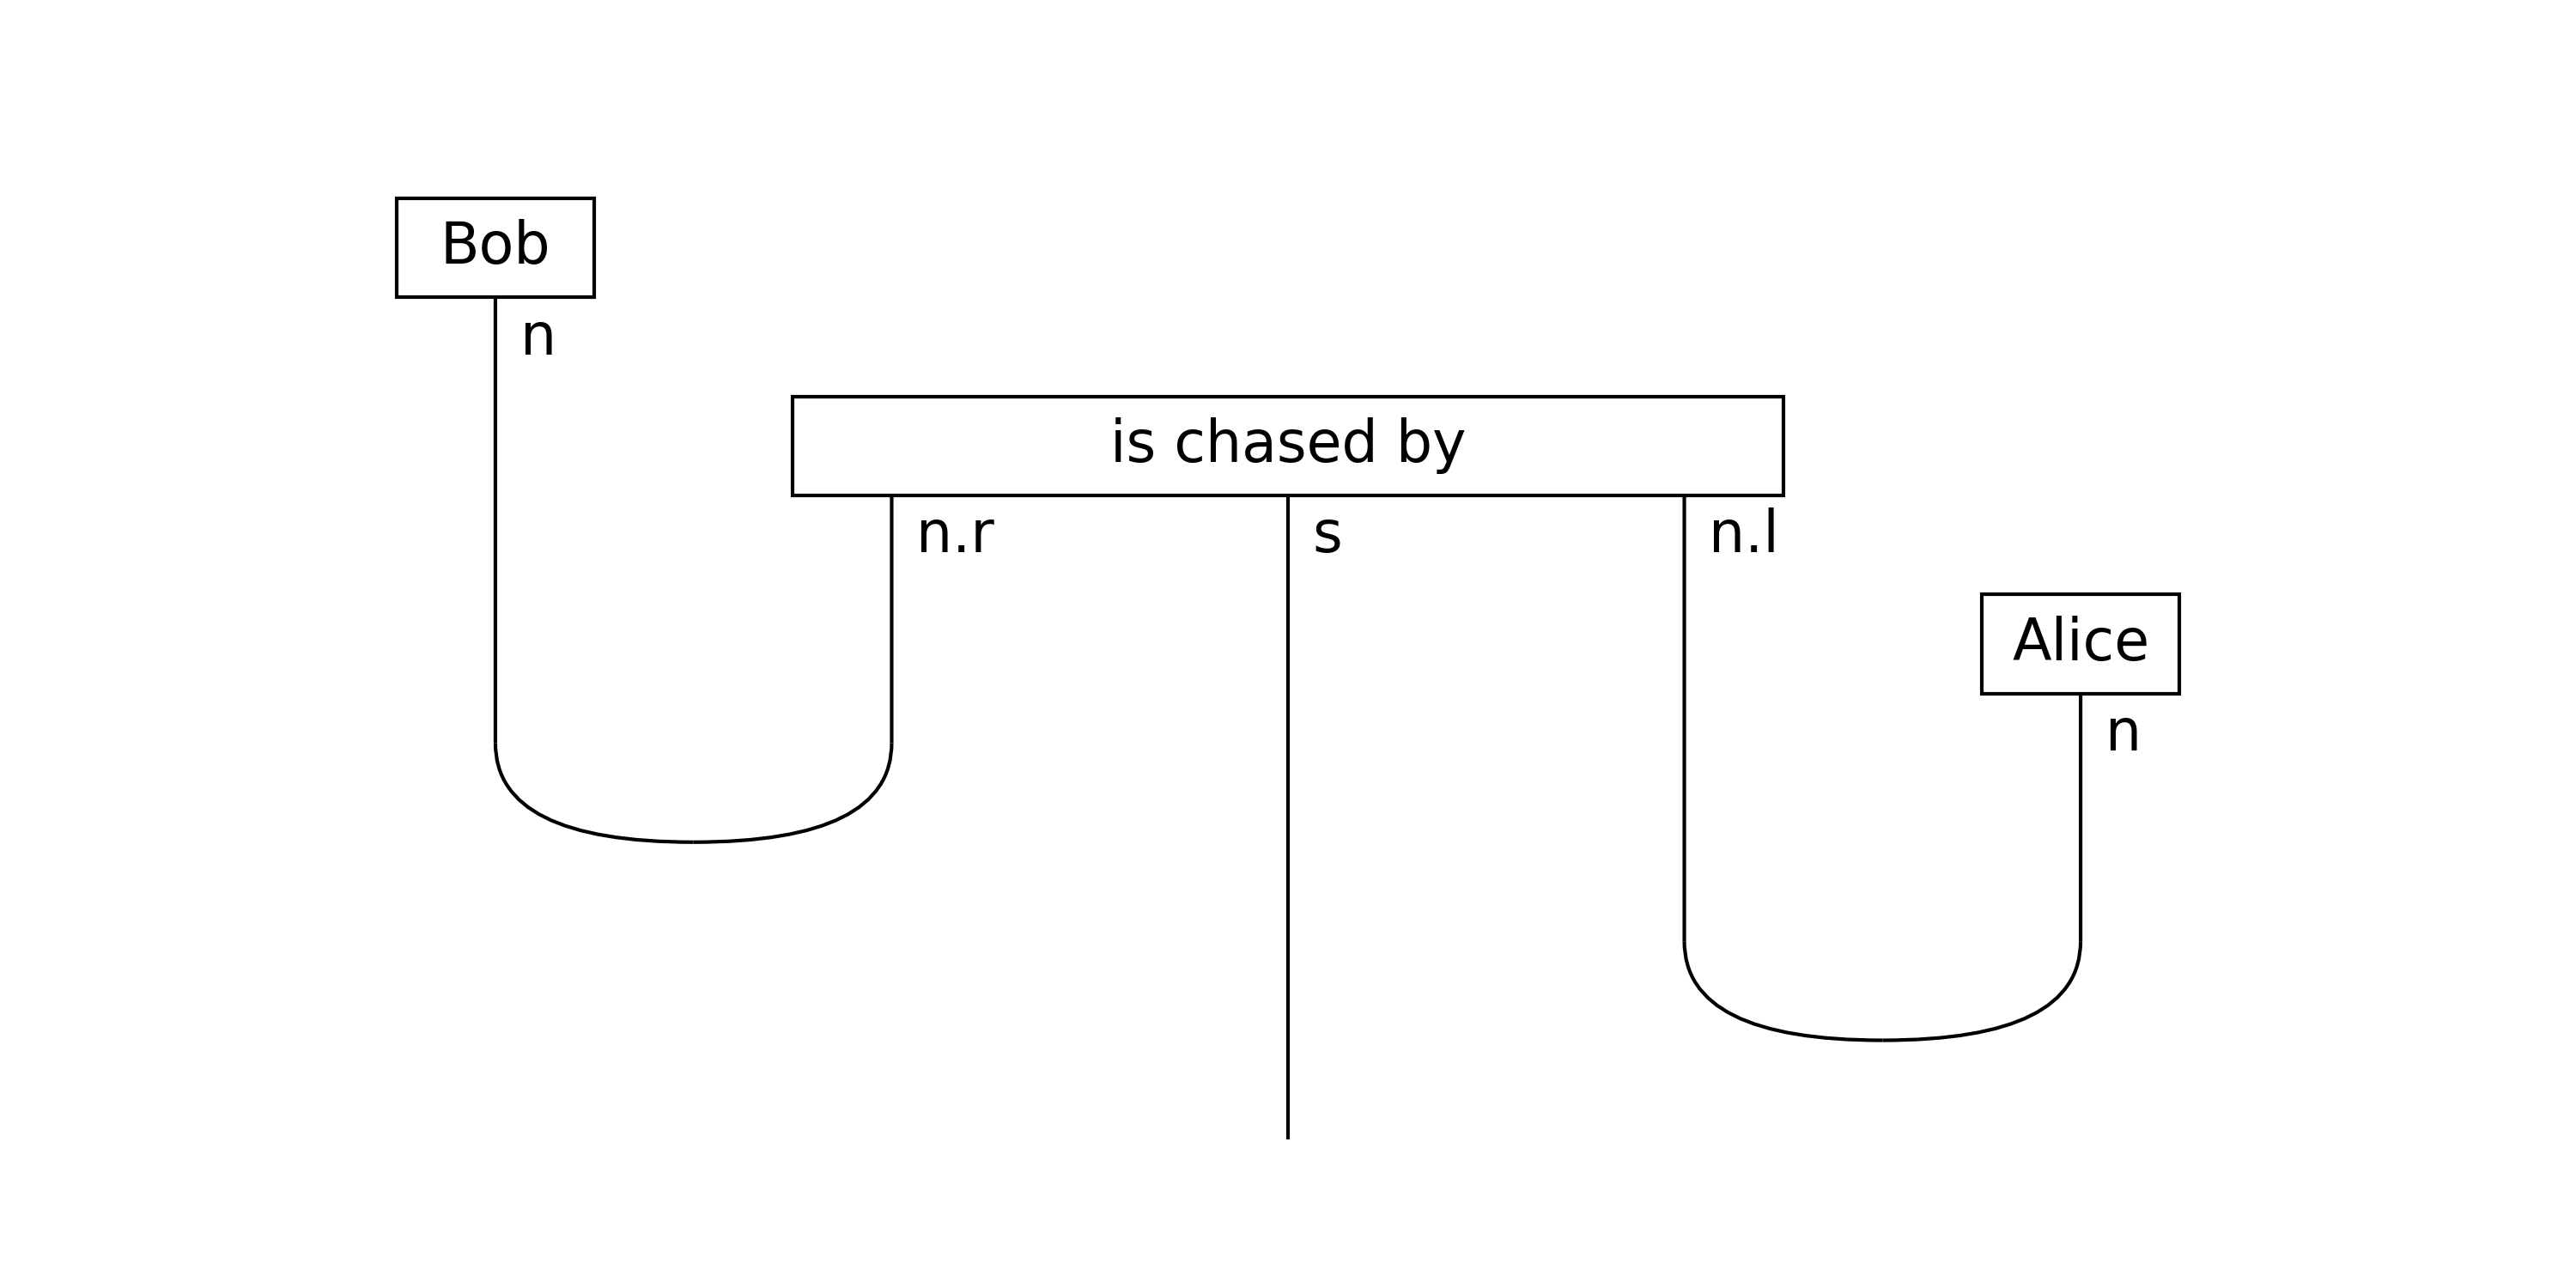
\includegraphics[keepaspectratio,alt={Passivization as role reassignment in the DisCoPy pregroup diagram for ``Bob is chased by Alice'' with type n\_\{\textbackslash text\{NOM\}\} \textbackslash otimes (n\^{}r \textbackslash otimes s \textbackslash otimes n\^{}l) \textbackslash otimes n\_\{\textbackslash text\{OBL\}\} \textbackslash to s. Bob's n wire contracts into the verb's left adjoint n\^{}r via the left Cup (n--n\^{}r) --- promoting the semantic patient to grammatical subject --- while Alice's n wire contracts into the right adjoint n\^{}l via the right Cup (n\^{}l--n), now demoted to the oblique by-phrase. Compare with  (active ``Alice chases Bob''), where Alice occupies the left subject slot and Bob the right object slot: the reassignment of which noun lands in each Cup is what makes voice alternation a topological swap \textbackslash sigma\_\{n,n\}\textbackslash colon n \textbackslash otimes n \textbackslash to n \textbackslash otimes n rather than a lexical substitution. Cup count is unchanged (two, matching the transitive active), so \textbackslash kappa(D) tracks argument slots rather than surface case marking; per  only the box count distinguishes the two diagrams (the passive inserts the ``is chased by'' box in place of the active ``chases'' box).}]{../figures/discopy_passive.png}}
\caption{Passivization as role reassignment in the DisCoPy pregroup
diagram for ``Bob is chased by Alice'' with type
\(n_{\text{NOM}} \otimes (n^r \otimes s \otimes n^l) \otimes n_{\text{OBL}} \to s\).
Bob's \(n\) wire contracts into the verb's left adjoint \(n^r\) via the
left Cup (\(n\)--\(n^r\)) --- promoting the semantic patient to
grammatical subject --- while Alice's \(n\) wire contracts into the
right adjoint \(n^l\) via the right Cup (\(n^l\)--\(n\)), now demoted to
the oblique \emph{by}-phrase. Compare with
\autoref{fig:discopy-discocat} (active ``Alice chases Bob''), where
Alice occupies the left subject slot and Bob the right object slot: the
reassignment of \emph{which} noun lands in each Cup is what makes voice
alternation a topological swap
\(\sigma_{n,n}\colon n \otimes n \to n \otimes n\) rather than a lexical
substitution. Cup count is unchanged (two, matching the transitive
active), so \(\kappa(D)\) tracks argument slots rather than surface case
marking; per \autoref{eq:eq-4-4} only the box count distinguishes the
two diagrams (the passive inserts the ``is chased by'' box in place of
the active ``chases'' box).}\label{fig:discopy-passive}
\end{figure}

Relative to \autoref{eq:eq-4-4}, the passive ``Bob is chased by Alice''
diagram in \autoref{fig:discopy-passive} has the same cup count as the
transitive active and therefore nearly identical \(\kappa(D)\); the
syntactic reassignment is visible in \emph{which} cup each noun enters,
not in the total count of contractions.
\end{frame}

\end{document}
